\chapter{Document Inserts}
\label{chap:inserts}
The remainder of this thesis comprises inserts from two documents:
\begin{itemize}
    \item \textbf{\ref{chap:inserts}.1} provides Chapter 2 from the
        documentation of version 2.0 of \acs{EsPy}. This chapter comprises
        tutorials describing how to use the
        package's \ac{API} for the consideration of \ac{1D} and \ac{2DJ}
        \ac{NMR} datasets. These tutorials provide a short description of the
        key features associated with the package, and is an ideal
        initial point of reference for new users to gain familiarity with
        \ac{EsPy}.
    \item \textbf{\ref{chap:inserts}.2} provides the current state of a draft
        for a paper to be submitted to \textit{Angewandte Chemie}, which
        outlines the methodology and results acquired using \ac{CUPID}.
\end{itemize}

\stepcounter{section}
\phantomsection
\addcontentsline{toc}{section}{\protect\numberline{\thesection}\acs{EsPy} Tutorials}
\sectionmark{\acs{EsPy} Tutorials}
\stepcounter{subsection}
\phantomsection
\addcontentsline{toc}{subsection}{\protect\numberline{\thesection}1D Tutorial}
\includepdf[%
    pages={13-19},%
    pagecommand={\thispagestyle{fancy}},%
    offset=0 -1cm,%
]{espy-docs.pdf}

\phantomsection
\stepcounter{subsection}
\phantomsection
\addcontentsline{toc}{subsection}{\protect\numberline{\thesection}2DJ Tutorial}
\includepdf[%
    pages={20-27},%
    pagecommand={\thispagestyle{fancy}},%
    offset=0 -1cm,%
]{espy-docs.pdf}
\clearpage
\stepcounter{section}
\sectionmark{\acs{CUPID} Paper Draft}
\phantomsection
\addcontentsline{toc}{section}{\protect\numberline{\thesection}\acs{CUPID} Paper Draft}
\label{sec:cupid-draft}
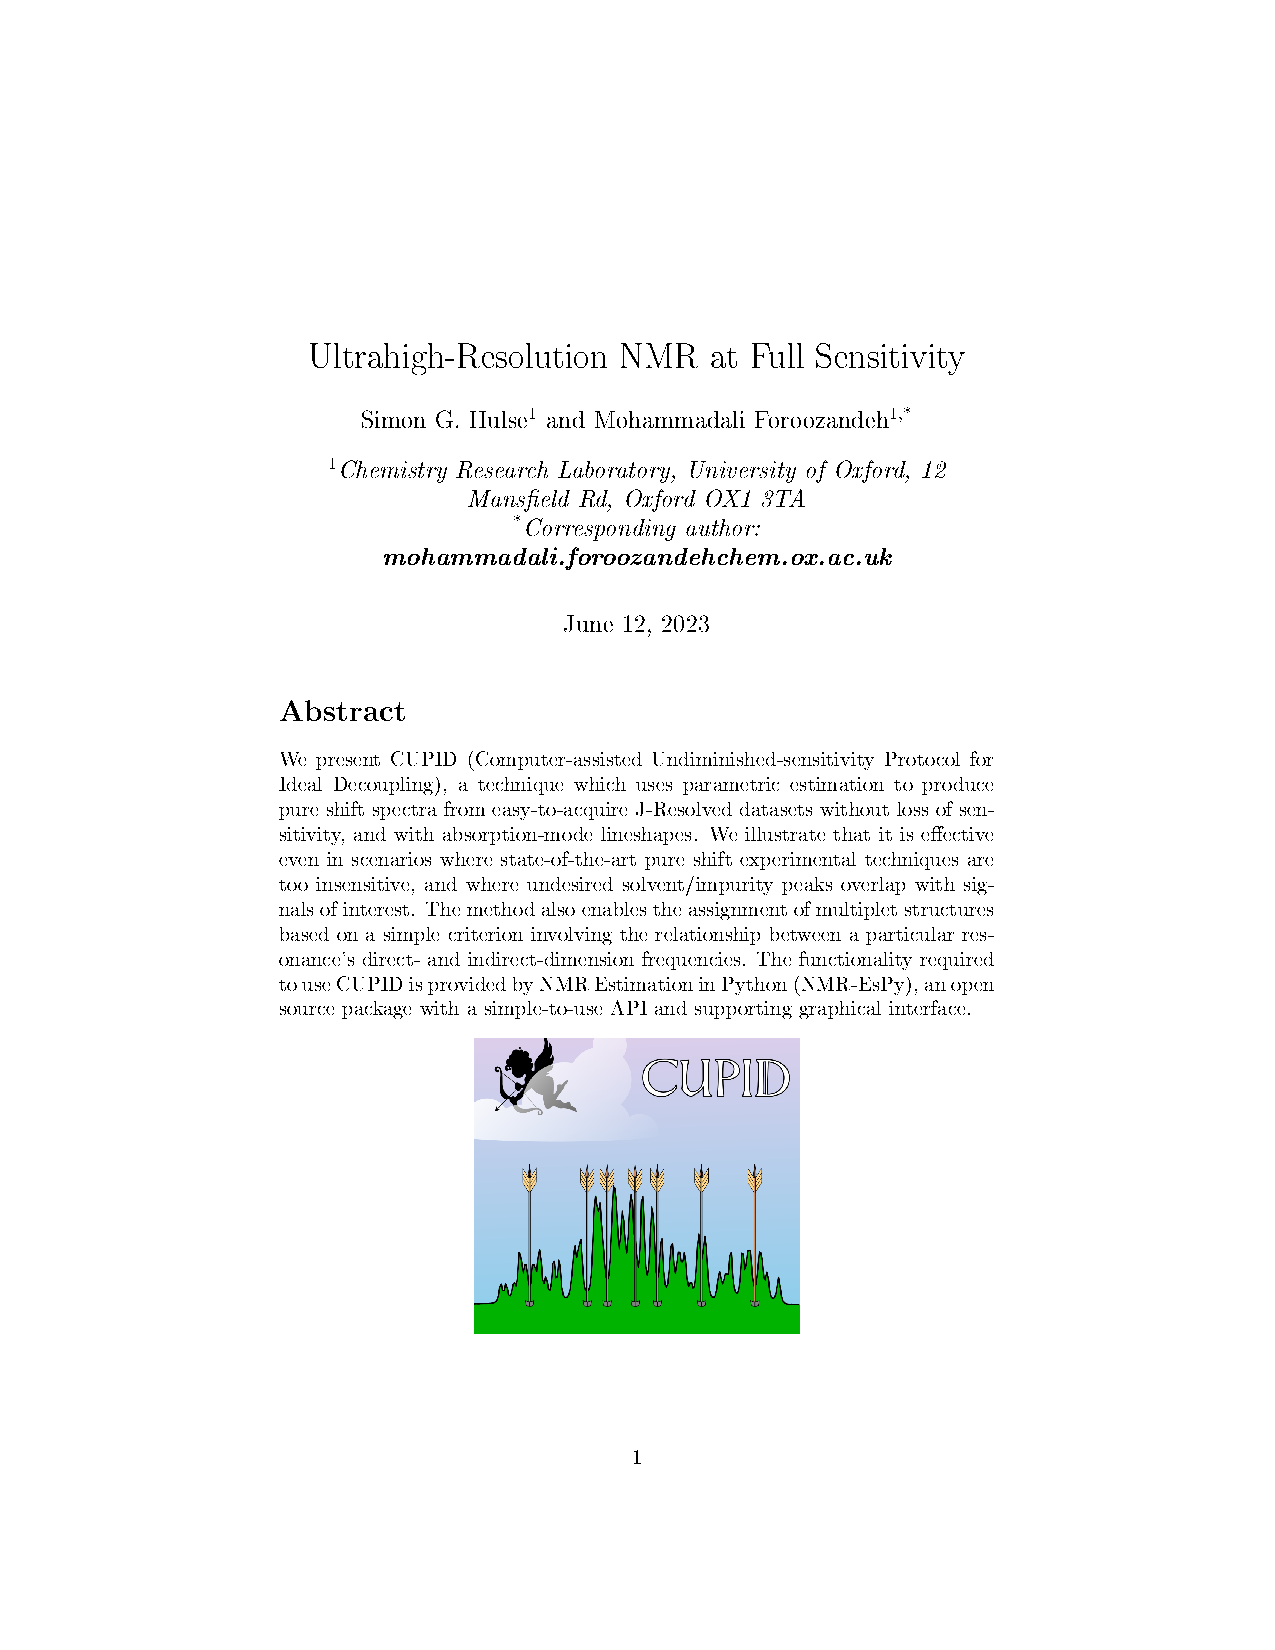
\includepdf[%
    pages=-,
    scale=0.9,%
    pagecommand={\thispagestyle{fancy}},%
    offset=0 -1cm,%
]{cupid-draft.pdf}
